% Chapter 10: Prediction and Confirmation
\chapter{Prediction and Confirmation}\label{sec:ch10-prediction}\label{chap:10}

An optimization ends with a recommended setting of the factors, but the recommendation is only as good as the model
behind it. The \ui{Prediction \& Confirmation} page (navigation group \ui{Optimization}) answers two questions:
\begin{enumerate}
  \item What does the model predict at a chosen setting, and how precise is that prediction?
  \item After new runs have been made at that setting, do the results agree with the prediction (is the model
    confirmed)?
\end{enumerate}
The examples use the case study \ui{Extraction Optimization (Box-Behnken)} (\menupath{File $\rightarrow$ Case
Studies\dots}): three factors (A: Temperature 60--80~°C, B: Time 30--90~min, C: Concentration 1--3~\%), 17 runs
with 5 center points, and the responses Yield (\%) and Purity (\%), each fitted with the quadratic model on the
\ui{RSM Analysis} page.

\section{The page}\label{sec:ch10-page}

The left side has two groups and a button (Figure~\ref{fig:ch10-prediction}):
\begin{itemize}
  \item \ui{Prediction Point (Actual Units)}: one input per factor, labeled with the factor name and unit. Numeric
    factors use a spin box whose range extends one factor range beyond the design (or data) limits on each side,
    so extrapolation is possible but is flagged. Categorical factors use a list of their levels. For a mixture, a
    line ``Component sum = \dots{} (must be \dots)'' turns red when the components do not add up to the mixture
    total.
  \item \ui{Options}: \ui{Confidence level:} and \ui{Number of confirmation runs (n):}
    (Table~\ref{tab:ch10-options}).
  \item \ui{Reset to Center Point}: sets every numeric factor to the center of its range (coded 0), every
    categorical factor to its first level, and mixture components to the mean of the design. This is also the
    starting point when a project is opened.
\end{itemize}
The right side holds the results table, a warning line in red above it and an explanation below it: CI and PI,
the confirmation rule, the scale of the standard error for transformed and for binomial or Poisson responses, the
note ``Typed confirmation means are cleared when a different point is sent to this page.'' and the confirmation rule
of an ANN. All values are recomputed as soon as an input or an option changes.

\begin{table}[htbp]
\centering
\caption{Options of the \ui{Prediction \& Confirmation} page.}\label{tab:ch10-options}
\begin{tabularx}{\linewidth}{@{}p{4.6cm}p{2.2cm}p{1.4cm}X@{}}
\toprule
Option & Values & Default & Meaning \\
\midrule
\ui{Confidence level:} & 90~\%, 95~\%, 99~\% & 95~\% & Level $1-\alpha$ of the confidence and prediction
  intervals. \\
\ui{Number of confirmation runs (n):} & 1--100 & 3 & Number of new runs whose \emph{mean} will be compared with the
  prediction; sets the width of the prediction interval. \\
\bottomrule
\end{tabularx}
\end{table}

\paragraph{Results table.} One row per response with the columns \ui{Response}, \ui{Prediction}, \ui{Std. Error of
mean}, \ui{CI low}, \ui{CI high}, \ui{PI low}, \ui{PI high}, \ui{Confirmation mean} and \ui{Status}. The response
name ends with ``[ANN]'' when the response is predicted by its neural network (Section~\ref{sec:ch10-ann});
otherwise the model of the \ui{RSM Analysis} page is used. Only \ui{Confirmation mean} can be edited. A dash
(``-'') marks a value that the model cannot provide.

\paragraph{Warnings.} The red line above the table shows any of:
\begin{itemize}
  \item ``The component sum does not equal the mixture total.''
  \item ``This point violates the component bounds / constraints.''
  \item ``The point is outside the design region - the prediction is an extrapolation.'' (process factors: a coded
    value is beyond $\pm1$ and beyond the largest coded value in the data).
\end{itemize}
A prediction with a warning can still be computed, but it should not be trusted without confirmation runs.

\paragraph{Data export.} Right-click the table to copy it (for Excel) or to save it with \ui{Export table\dots}
as an Excel or CSV file.

\section{Predicting at a chosen setting}\label{sec:ch10-predict}

\subsection{How to use}

\begin{enumerate}
  \item Open \ui{Prediction \& Confirmation}.
  \item Type the factor settings in actual units in \ui{Prediction Point (Actual Units)}, or send a solution from
    an optimization page (Section~\ref{sec:ch10-send}).
  \item Choose the confidence level and the number $n$ of confirmation runs you plan to make.
  \item Read the prediction and its intervals in the table.
\end{enumerate}

\subsection{Theory as implemented (RSM)}\label{sec:ch10-theory}

For a least-squares model with model matrix $\mathbf{X}$ ($N$ runs, $p$ coefficients), coefficient estimates
$\mathbf{b}$, residual mean square $\text{MSE}$ and residual degrees of freedom $\nu_\text{E} = N - p$, let
$\mathbf{x}_0$ be the model row of the chosen point (the coded factors expanded into the model terms). Then
\citep{montgomery2017,myers2016}
\begin{align}
  \hat y_0 &= \mathbf{x}_0^\top \mathbf{b}, \qquad
  h_0 = \mathbf{x}_0^\top \left(\mathbf{X}^\top\mathbf{X}\right)^{-1} \mathbf{x}_0, \label{eq:ch10-pred}\\
  \text{SE}_\text{mean} &= \sqrt{\text{MSE}\; h_0}, \qquad
  \text{SE}_{\text{pred},n} = \sqrt{\text{MSE}\left(\frac{1}{n} + h_0\right)}, \label{eq:ch10-se}\\
  \text{CI}:&\quad \hat y_0 \pm t_{1-\alpha/2,\,\nu_\text{E}}\; \text{SE}_\text{mean}, \label{eq:ch10-ci}\\
  \text{PI}:&\quad \hat y_0 \pm t_{1-\alpha/2,\,\nu_\text{E}}\; \text{SE}_{\text{pred},n}. \label{eq:ch10-pi}
\end{align}
The quantity $h_0$ is the scaled prediction variance of the point; it is small near the center of the design and
grows toward its edges and beyond.
\begin{itemize}
  \item The \emph{confidence interval} (CI) covers the true \emph{mean} response at the point. Its width depends only
    on how well the model is estimated there.
  \item The \emph{prediction interval} (PI) covers the \emph{mean of $n$ new runs} at the point. It adds the
    variance $\text{MSE}/n$ of that mean to the uncertainty of the model, so it is always wider than the CI. With
    $n = 1$ it is the usual interval for a single new observation; as $n$ grows it shrinks toward the CI.
\end{itemize}
The interval assumes that the model is correct at the point, that the errors are independent with constant
variance, and that the new runs are made under the same conditions as the experiment. If the model has no residual
degrees of freedom ($\nu_\text{E} = 0$), no intervals can be computed and the cells show ``-''. In a design with
blocks, the prediction is for the average over the blocks (the block effects are set to zero).

\paragraph{Transformed responses.} If a transformation (for example ln or square root) is selected for the
response on the \ui{RSM Analysis} page, the model is fitted to $z = g(y)$. The prediction and the interval limits are
computed on the transformed scale and converted back with $g^{-1}$:
\begin{equation}
  \hat y_0 = g^{-1}(\hat z_0), \qquad
  \left[\min\!\left(g^{-1}(z_\text{lo}), g^{-1}(z_\text{hi})\right),\;
        \max\!\left(g^{-1}(z_\text{lo}), g^{-1}(z_\text{hi})\right)\right].
  \label{eq:ch10-back}
\end{equation}
The back-transformed intervals are therefore not symmetric about the prediction. The column \ui{Std. Error of
mean} is \emph{not} back-transformed: it is the standard error of $\hat z_0$ and is labeled ``(transformed scale)''
(the tooltip of the cell explains this). For an ln transform it is approximately the relative standard error of the
prediction. Note also that the back-transformed prediction estimates the median of the response rather than its
mean when the transformation is nonlinear (for ln, the mean is larger than the median).

\paragraph{Other kinds of models.} For a split-plot design analyzed by REML, the prediction interval of the mean of
$n$ new runs also contains the whole-plot variance: $\text{SE}_{\text{pred},n} = \sqrt{h_0 + \sigma^2_\text{WP} +
\sigma^2/n}$, where $h_0$ is already on the variance scale, and the $t$ quantile uses the residual degrees of
freedom of the split-plot analysis. For a binomial or Poisson response (logistic or Poisson regression), the confidence interval
is a Wald interval on the link scale with a normal quantile, transformed to a proportion or a count; there is no
prediction interval. \ui{Std. Error of mean} is then the standard error of the linear predictor and is labeled
``(link scale, logit)'' or ``(link scale, log)''; its tooltip reads ``Standard error of the linear predictor on the
link scale (logit); the CI is converted back to the response scale.'' (with ``log'' for Poisson).

\subsection{Example: the best desirability solution}

On the \ui{Desirability} page, with Yield and Purity both maximized, the best solution is Temperature 70.265~°C,
Time 89.781~min and Concentration 1.7975~\% (coded $0.027$, $0.993$, $-0.203$). It was sent to the prediction page
with \ui{Send Selected Solution to Prediction}; Figure~\ref{fig:ch10-prediction} shows the result at 95~\% with
$n = 3$.

For Yield, the quadratic model has $p = 10$ coefficients, $\nu_\text{E} = 7$ and $\text{MSE} = 0.5092$; at this
point $h_0 = 0.3633$ and $t_{0.975,7} = 2.3646$. Equations~\eqref{eq:ch10-pred}--\eqref{eq:ch10-pi} give
\begin{align*}
  \hat y_0 &= 78.290, \qquad \text{SE}_\text{mean} = \sqrt{0.5092 \times 0.3633} = 0.4301,\\
  \text{CI} &= 78.290 \pm 2.3646 \times 0.4301 = [77.273,\ 79.307],\\
  \text{SE}_{\text{pred},3} &= \sqrt{0.5092\,(1/3 + 0.3633)} = 0.5956,\\
  \text{PI} &= 78.290 \pm 2.3646 \times 0.5956 = [76.882,\ 79.698].
\end{align*}
For Purity ($\text{MSE} = 0.1385$, same $h_0$ and $t$), the prediction is 92.416 with $\text{SE}_\text{mean} =
0.2243$, CI $[91.886, 92.946]$ and PI $[91.682, 93.151]$.

The leverage $h_0 = 0.363$ is much larger than at the design center ($h_0 = 0.200$) because the optimum lies at the
upper edge of the Time range. At the center the Yield CI is $77.772 \pm 0.755$; at the optimum it is $\pm 1.017$.
Optima often lie at the edge of the design region, where the model is least precise.

\begin{figure}[htbp]
\centering
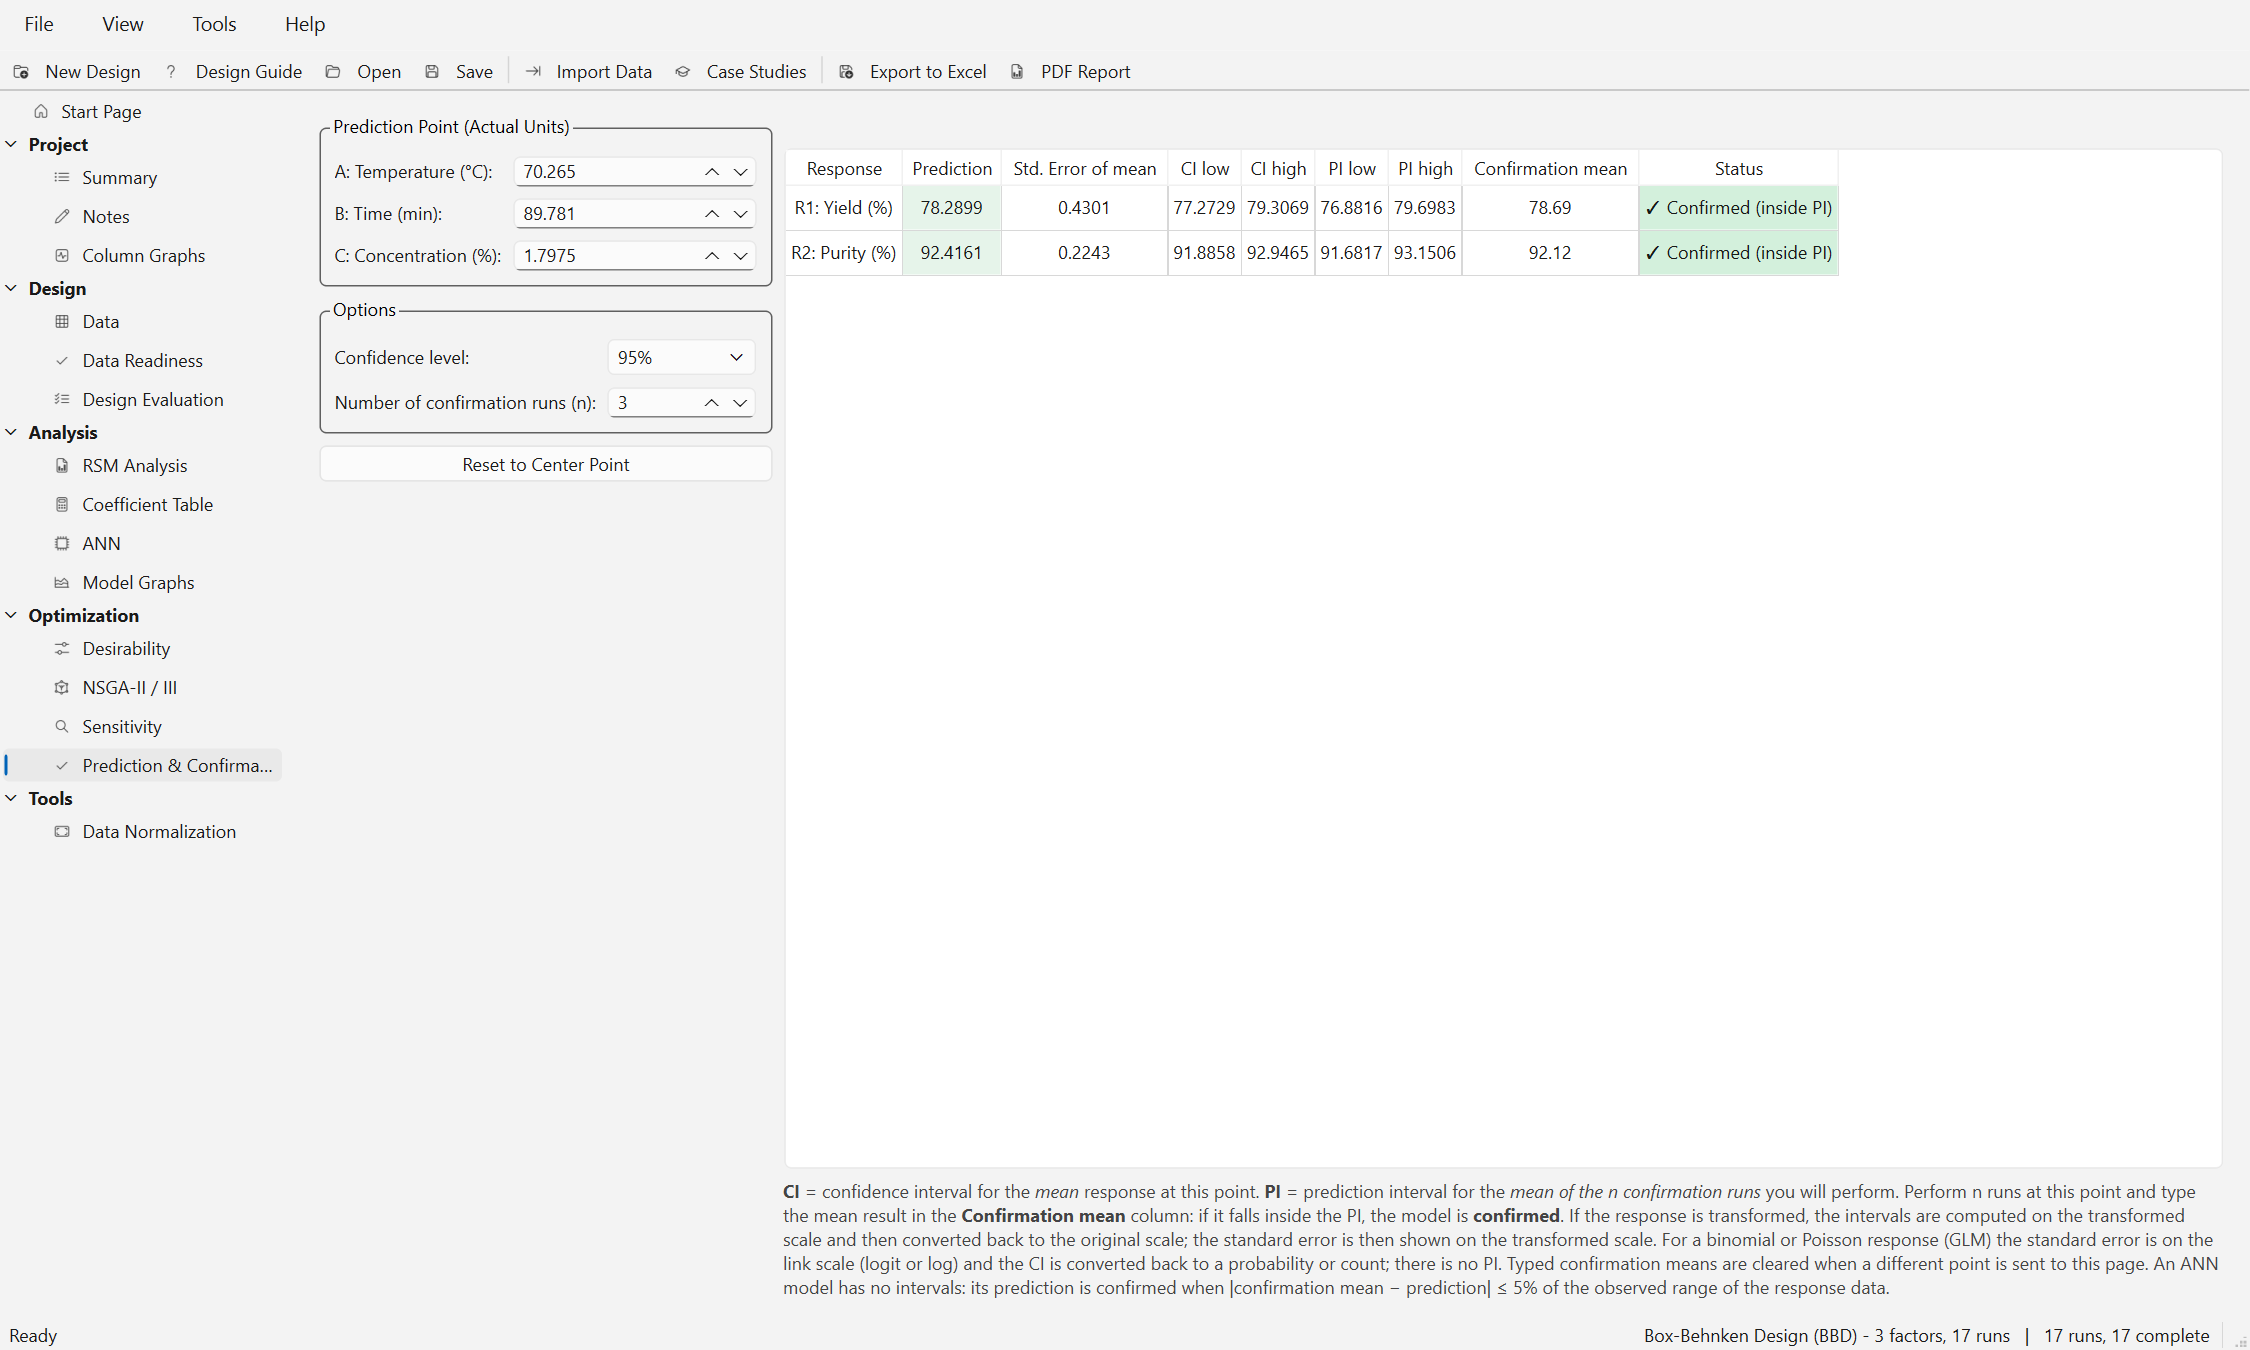
\includegraphics[width=\linewidth]{prediction.png}
\caption{\ui{Prediction \& Confirmation} page with the best desirability solution of the extraction case (95~\%,
$n = 3$). The confirmation means 78.69 (Yield) and 92.12 (Purity) lie inside the prediction intervals: both
responses are confirmed.}
\label{fig:ch10-prediction}
\end{figure}

\section{Predicting with an ANN}\label{sec:ch10-ann}

When the box \ui{Use this response's ANN for graphs, optimization, NSGA-II \& prediction} is ticked on the
\ui{ANN} page (or ANN is chosen in the \ui{Model} column of an optimization page), the response is predicted by its
network and its name ends with ``[ANN]''. The network gives only the point prediction (Eqs.~\eqref{eq:ch07-input}--\eqref{eq:ch07-output} in
Chapter~\ref{chap:7}, with the normalization converted back to response units):
\begin{itemize}
  \item available: \ui{Prediction};
  \item not available (shown as ``-''): \ui{Std. Error of mean}, the CI and the PI. A neural network fitted by
    REGEN has no standard error or interval, because its parameters are not estimated by a linear model with known
    sampling distribution.
\end{itemize}
The uncertainty of an ANN prediction is best judged from the cross-validated test RMSE of the architecture search
(Chapter~\ref{chap:7}): it is the typical error to expect at a new point inside the region covered by the data. For the dye
adsorption network of Chapter~\ref{chap:7} it is 4.07 percentage points of removal efficiency. Outside that region, or in
gaps between the runs, the error can be much larger.

\section{Sending solutions from the optimization pages}\label{sec:ch10-send}

Instead of typing a point, send it from an optimization:
\begin{itemize}
  \item \ui{Desirability}: select a row of the solutions table and click \ui{Send Selected Solution to
    Prediction}.
  \item \ui{NSGA-II / III}: select a Pareto solution and click \ui{Send Selected Solution to Prediction}; without a
    selection the TOPSIS compromise solution is sent.
\end{itemize}
The page opens with the factor inputs set to the solution. Each response is predicted with the model selected for
it (RSM or ANN), as in the optimization. Values typed earlier in \ui{Confirmation mean} belong to the previous point:
they are cleared when a different point is sent to the page (also by \ui{Reset to Center Point} when the point was
not already the center), and kept when the same point is sent again. (When you
change the factor inputs by hand, the typed values stay and are judged against the new prediction; clear them
yourself in that case.)

\section{Confirmation runs}\label{sec:ch10-confirm}

\subsection{How to use}

\begin{enumerate}
  \item Choose the point and set \ui{Number of confirmation runs (n):} to the number of runs you will make.
  \item Make the $n$ runs at the point (Section~\ref{sec:ch10-advice}) and compute the mean result of each response.
  \item Type the mean in the \ui{Confirmation mean} column of each response. A decimal point or a decimal comma may
    be used.
  \item Read the \ui{Status} column.
\end{enumerate}
Confirmation values are kept while the project is open but are not saved in the project file. Record them in the
\ui{Notes} page or in the data table if they should be kept.

\subsection{Confirmation rules}

\paragraph{RSM model.} The model is confirmed when the mean of the $n$ runs falls inside the prediction interval
for the mean of $n$ runs, Eq.~\eqref{eq:ch10-pi}:
\begin{equation}
  \text{PI}_\text{low} \le \bar y_\text{conf} \le \text{PI}_\text{high}. \label{eq:ch10-rule-rsm}
\end{equation}
The status is ``\checkmark{} Confirmed (inside PI)'' on a green background or ``$\times$ Outside PI'' on a red one.
For binomial and Poisson responses only the CI exists, and the statuses are ``Confirmed (inside CI)'' and ``Outside
CI''. A value that cannot be read gives ``Not a number''.

At the confidence level $1-\alpha$, a correct model gives a confirmation mean outside the PI with probability
$\alpha$ (5~\% at the default level). A single result outside the PI is therefore evidence, not proof, that the model
is wrong at this point, and a result inside it does not prove the model correct elsewhere.

\paragraph{ANN model.} Because a network has no prediction interval, its prediction is confirmed when the
difference is small compared with the spread of the response in the data:
\begin{equation}
  \left|\bar y_\text{conf} - \hat y_0\right| \le 0.05\,\left(y_\text{max} - y_\text{min}\right),
  \label{eq:ch10-rule-ann}
\end{equation}
where $y_\text{max}$ and $y_\text{min}$ are the largest and smallest values of the response among the runs used for
modeling. The status reads, for example, ``\checkmark{} Error 1.676 = 3.01\% of the data range ($\le$ 5\%)''
or ``$\times$ Error \dots{} (> 5\%)''. (If all response values are equal, the relative error $|\bar y_\text{conf} -
\hat y_0|/|\hat y_0|$ is used instead with the same 5~\% limit.)

This rule is an engineering tolerance, not a statistical test. It ignores the number of runs and the noise of the
measurement. If the pure-error standard deviation is large compared with 5~\% of the range, even a perfect model
will often fail it with $n = 1$; if the range is very wide, it is lenient. Compare the tolerance with the noise
before relying on it: in the extraction case, 5~\% of the Yield range (64.13 to 78.29) is 0.71, about twice the
pure-error standard deviation of 0.34, so a mean of three runs (standard error $0.34/\sqrt3 = 0.20$) is a fair test.

\paragraph{Example (RSM).} In Figure~\ref{fig:ch10-prediction}, the means of three confirmation runs are 78.69 for
Yield and 92.12 for Purity. Both lie inside their PIs, $[76.88, 79.70]$ and $[91.68, 93.15]$, so both responses are
confirmed. A Yield mean of 80 would be outside the PI and shown as ``Outside PI''.

\paragraph{Example (ANN).} For the dye adsorption case with the 4-3-1 network of Chapter~\ref{chap:7} selected, the
prediction at the center of the factor space (pH 6, Adsorbent Dose 2.25~g/L, Contact Time 65~min, Initial
Concentration 110~mg/L) is 40.82~\%. The response range in the data is $58.45 - 2.73 = 55.72$, so the tolerance is
$0.05 \times 55.72 = 2.79$: a confirmation mean between 38.04 and 43.61 confirms the network. A mean of 42.5 gives
an error of 1.676, which is 3.01~\% of the range, and is accepted.

\subsection{What to do when a confirmation fails}

\begin{enumerate}
  \item Check the runs: were the factor settings, the measurement and the material the same as in the experiment?
    A drift in raw material or equipment shifts all new results.
  \item Check whether the point was an extrapolation or lay in a sparse part of the factor space (warning line,
    \ui{Data Readiness} page, ANN data adequacy).
  \item Add the confirmation runs to the data as ordinary runs and refit the model. Several confirmation points
    around the optimum also improve the model where it matters most (the \ui{Data Readiness} page can suggest them).
  \item If the model is systematically wrong (lack of fit on the \ui{RSM Analysis} page), consider a higher-order
    model, a transformation or an ANN; if the ANN fails, consider RSM or more runs (learning curve, Chapter~\ref{chap:7}).
  \item Repeat the optimization with the refitted model and confirm again.
\end{enumerate}

\section{Planning confirmation runs}\label{sec:ch10-advice}

\paragraph{Number of runs.} The prediction interval narrows as $n$ grows, but never below the confidence interval.
For Yield at the desirability solution (95~\%):

\begin{table}[htbp]
\centering
\caption{Prediction interval for the mean of $n$ confirmation runs, Yield at the best desirability solution.}
\label{tab:ch10-n}
\begin{tabular}{@{}lccc@{}}
\toprule
$n$ & $\text{SE}_{\text{pred},n}$ & PI & Half width \\
\midrule
1 & 0.833 & $[76.32,\ 80.26]$ & 1.97 \\
3 & 0.596 & $[76.88,\ 79.70]$ & 1.41 \\
5 & 0.536 & $[77.02,\ 79.56]$ & 1.27 \\
$\infty$ (CI) & 0.430 & $[77.27,\ 79.31]$ & 1.02 \\
\bottomrule
\end{tabular}
\end{table}

Going from one to three runs narrows the interval by 28~\%; going further gains little, because the uncertainty of
the model itself ($h_0$) then dominates. Three to five runs are usually a good compromise. Set
\ui{Number of confirmation runs (n):} to the number you actually make: the interval is valid only for the mean of
that many runs.

\paragraph{How to make the runs.} Confirmation runs must be genuine replicates: set the factors anew for each run,
run them in random order and, if possible, spread them over time, exactly as in the original experiment. Repeated
measurements of one batch are not independent runs and make the result look more precise than it is. Use the same
equipment, materials and measurement method as in the experiment.

\paragraph{Where to make the runs.}
\begin{itemize}
  \item At the recommended optimum, which is the point that matters.
  \item When the optimum lies at the edge of the region, also at a point slightly inside it, where the model is more
    precise.
  \item For a multi-objective optimization, at the TOPSIS compromise and, if the trade-off is still open, at one or
    two other Pareto solutions.
  \item When RSM and ANN disagree about the optimum (check~D, the comparison of the RSM and ANN Pareto fronts in
    Chapter~\ref{chap:8}: a mean prediction difference above 5~\% of the response range or compromise points more than 15~\%
    of the factor range apart), make confirmation runs at both TOPSIS points. The runs decide which model describes
    the process, and they add data where the models disagree.
\end{itemize}

\paragraph{Model choice.} For each confirmation point, look at the predictions of both models before the runs are
made (switch the model with the check box on the \ui{ANN} page or the \ui{Model} column on the optimization pages).
If the two predictions differ by more than the PI half width, the confirmation runs also tell which model to
use. Record the results and add them to the data set; they are the most valuable runs of the study.
